%!TEX root = <uw-ethesis.tex>
% T I T L E   P A G E
% -------------------
% Last updated May 24, 2011, by Stephen Carr, IST-Client Services
% The title page is counted as page `i' but we need to suppress the
% page number.  We also don't want any headers or footers.
\pagestyle{empty}
\pagenumbering{roman}

% The contents of the title page are specified in the "titlepage"
% environment.
\begin{titlepage}
        \begin{center}
        % \vspace*{1.0cm}

        \Large
        {\bf \sc \underline{University Of Waterloo}}
        
        \normalsize
        {\bf \sc Faculty Of Engineering \\
        Mechanical And Mechatronics Engineering} \\

        \vspace*{1.0cm}
        \Large
        {\bf \uppercase{Video encoding techniques for networked low power applications}}
        
        \vspace*{1.5cm}
        \normalsize
        \begin{figure}[h!]
        \centering
        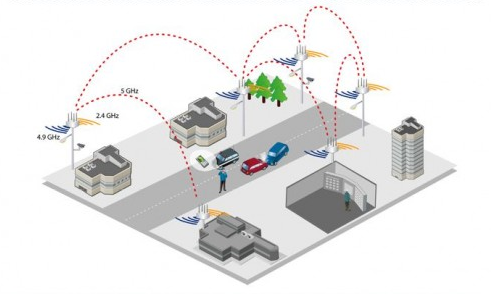
\includegraphics[width=\textwidth]{title}
        \label{fig:tit}
        \end{figure}
        
        \vfill
        {\sc Self Study Report}

        \vspace*{1cm}
        Prepared by\\
        {\sc Satya Prahlada Sthita Prajna Kandarpa \\
        UW ID 20402024 $\vert$ Userid \textit{spspkand} \\ 
        4B Mechatronics Engineering \\
        31 December 2015}

        \end{center}
\end{titlepage}



\cleardoublepage % Ends the current page and causes all figures and tables that have so far appeared in the input to be printed.
% In a two-sided printing style, it also makes the next page a right-hand (odd-numbered) page, producing a blank page if necessary.

% Letter of Submittal%
\begin{flushleft}
    41 Pineslope Crescent\\
    Scarborough, Ontario, Canada\\
    M1E 4M5
    
    31 December 2015
    
    Professor William Melek,\\
    Director of Mechatronics Engineering\\
    Department of Mechanical and Mechatronics Engineering\\
    University of Waterloo\\
    Waterloo, Ontario\\
    N2L 3G1
    
    Dear Sir,

    This report, titled "Video encoding techniques for networked low power applications", was prepared as my 4B Work Report for the University of Waterloo. This report is in fulfillment of the course WKRPT 400. The purpose of this report is to evaluate standard video encoding techniques in the context of networked low power video sensor applications and compare their performance with novel encoding techniques developed for distributed sensor networks.
    
    I got exposed to some innovative and novel media processing techniques at a startup I worked at which helped pique my interest in audio visual media processing. This report intends to provide guidance and critical technical evaluation from a software performance perspective to anyone interested in developing low power sensor networks that integrate cameras, audio sensors and mobile communication devices. 

    The technical analysis conducted by me for this purpose incorporates machine learning techniques to evaluate the standard video encoding technologies to produce optimized encoding parameters that may match the aforementioned specialized distributed video codecs in terms of video transcoding performance. This analysis maybe useful to anyone who would like to avoid the high license costs for the specialized video codecs.  
    
    This report was written entirely by me and has not received any previous academic credit at this or any other institution. 

    Sincerely,\\
    Satya Prahlada Sthita Prajna Kandarpa\\
    ID 20402024\\
\end{flushleft}
\cleardoublepage

